\section{Introduction}\label{introduction}

\begin{frame}{Basic Analyses}

\center
\textbf{Basic Analyses}: The analyses taught in the first stats course
\vspace{12pt}

\columnsbegin

\begin{column}{0.48\textwidth}
   These include:
   \begin{enumerate}
   \item T-tests
   \item ANOVA
   \item Linear Regression
   \end{enumerate}
   These allow us to assess relationships like that in the figure.
\end{column}\begin{column}{0.48\textwidth}
    \begin{center}
     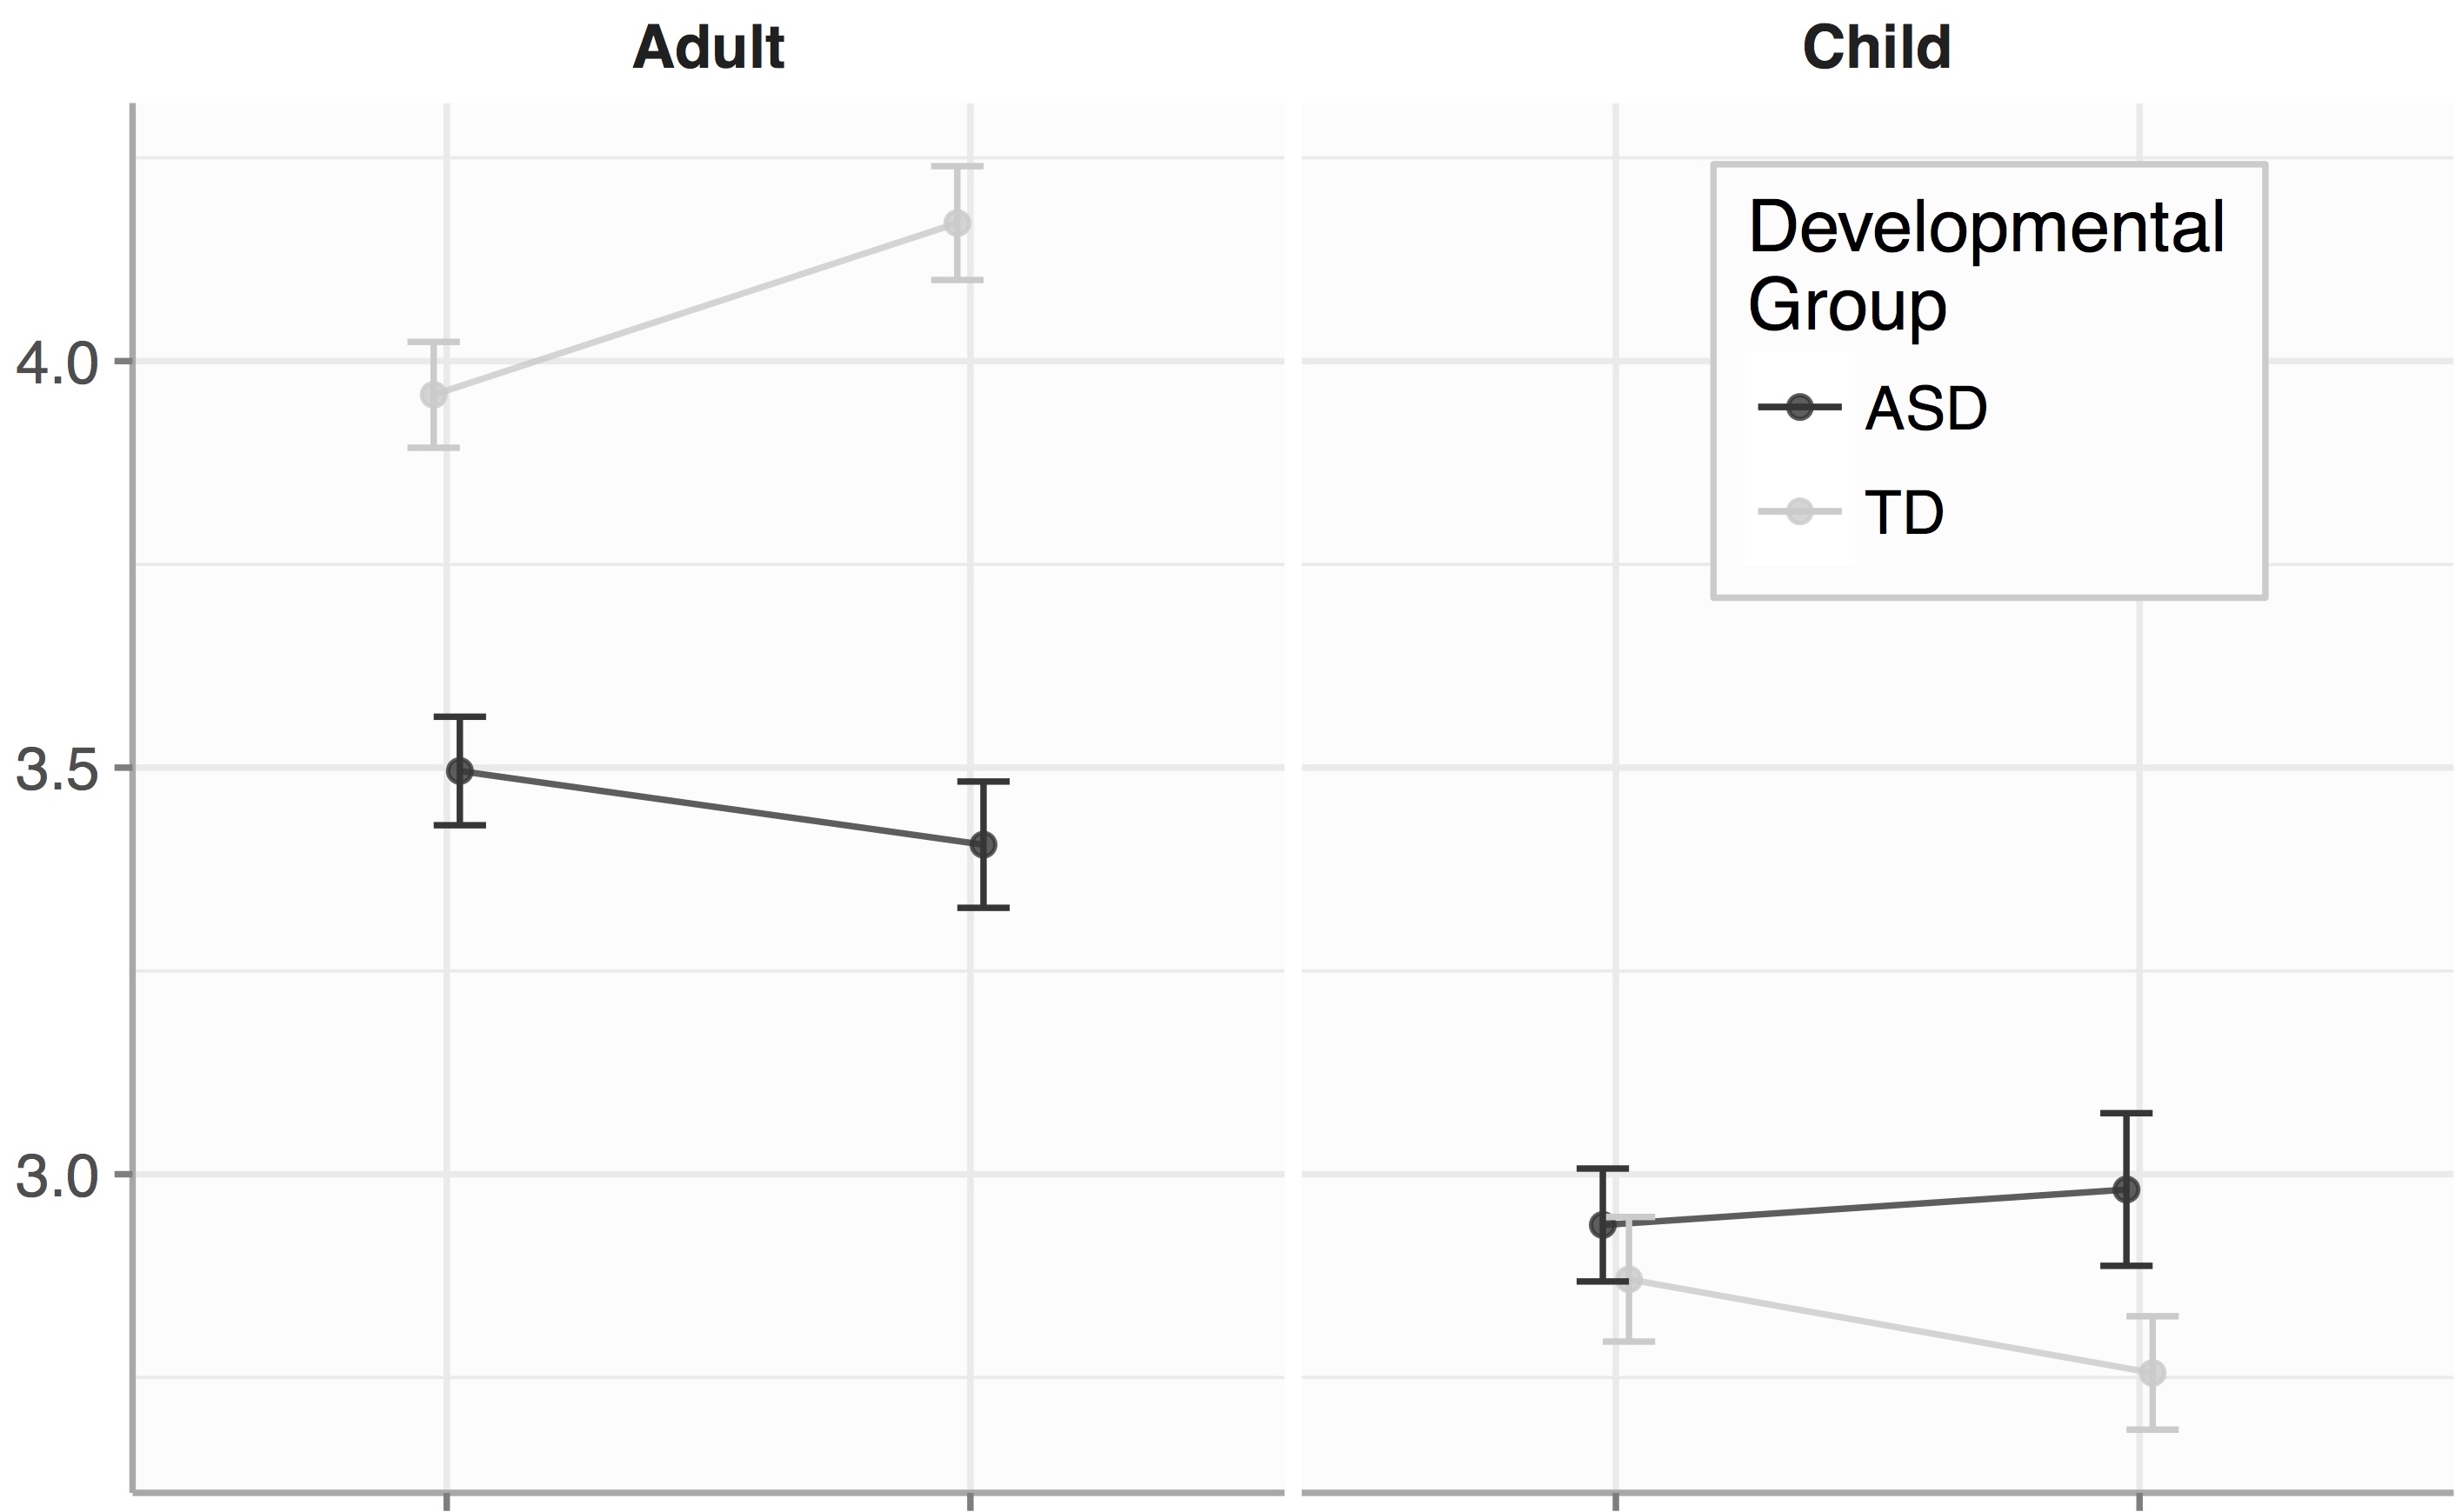
\includegraphics[width=\textwidth]{Figures/FigureInteraction.jpg}
     \end{center}
\end{column}

\columnsend

\vspace{12pt} Maybe surprising:\textbackslash{} These all are doing
essentially the same thing!

First, \textbf{T-TESTS!}

\end{frame}

\section{T-tests}\label{t-tests}

\begin{frame}{Three Types}

\Huge

\begin{enumerate}
\item Simple
\item Independent Samples
\item Paired Samples
\end{enumerate}

\end{frame}

\begin{frame}[fragile]{Three Types}

\Large
Each will be demonstrated using:

\normalsize

\begin{Shaded}
\begin{Highlighting}[]
\NormalTok{df <-}\StringTok{ }\KeywordTok{data.frame}\NormalTok{(}\StringTok{"A"}\NormalTok{=}\KeywordTok{sample}\NormalTok{(}\KeywordTok{c}\NormalTok{(}\DecValTok{0}\NormalTok{,}\DecValTok{1}\NormalTok{), }\DecValTok{100}\NormalTok{, }\DataTypeTok{replace =} \OtherTok{TRUE}\NormalTok{),}
                 \StringTok{"B"}\NormalTok{=}\KeywordTok{rnorm}\NormalTok{(}\DecValTok{100}\NormalTok{),}
                 \StringTok{"C"}\NormalTok{=}\KeywordTok{rnorm}\NormalTok{(}\DecValTok{100}\NormalTok{))}
\NormalTok{df}
\end{Highlighting}
\end{Shaded}

\begin{verbatim}
    A           B           C
1   1  0.10374689 -0.32650412
2   0  1.56780670  0.77258383
3   1 -0.67845631  1.48447975
4   0  1.66587597 -1.29542982
5   1 -0.14670047  0.17361789
6   0 -0.62734606 -0.14871939
7   1  1.34815779 -1.39987953
8   1 -0.91928687 -0.27870608
9   0 -0.27793293 -0.38088161
10  1 -0.35931289 -0.88442039
11  1 -0.58474750  1.24518287
12  1  0.41195278 -0.08099849
13  1 -0.49405468 -1.22595760
14  0  1.63740588 -0.91031483
15  1  1.58786455 -0.76847436
16  0 -0.61779190  1.87868273
17  0  0.14932852 -1.35604458
18  0 -1.38913186 -1.19088755
19  1 -2.36750379  0.05398181
20  1  1.50048801  0.48749654
21  1  1.74046502  0.54618107
22  0 -1.12655864  0.37696095
23  1  1.38190674  0.59639591
24  0  3.06371523  0.31713898
25  1 -1.01414188  1.06669614
26  1 -0.55129097  0.20043984
27  1 -3.03874906 -0.40125043
28  1  0.10155882 -0.19787223
29  0  0.96656724 -1.05555729
30  0 -1.03572243  0.02417963
31  1 -1.22103046 -0.63255770
32  1  1.25093140 -0.29939750
33  1 -1.35323789 -0.59496036
34  1 -0.33120508 -1.83379895
35  1  1.02852346  0.04301486
36  1 -0.91522665 -0.52700705
37  1  1.31019124 -0.76150267
38  1  0.33444865  0.84251046
39  1 -1.86108065 -0.76009730
40  1  0.76657668  0.50631656
41  0 -0.93326201 -0.05765941
42  0 -0.48219557 -0.54732691
43  1  0.28945514 -0.95762588
44  1  0.30474286 -1.67611135
45  1  1.24641517 -0.34660164
46  1 -0.30848966 -0.16268931
47  0  0.29545657  0.50293098
48  1 -0.59637823  0.18499430
49  0  0.05952506 -0.46526971
50  0 -0.18110056  0.70449814
51  1  0.03069989 -0.09867987
52  1  0.30266427 -0.71117668
53  0  1.15100114  0.08506981
54  1  0.13634888  0.07527945
55  0 -1.06927233  0.62035929
56  1  1.73836790  0.21619956
57  0  1.03004236  0.01911779
58  1  1.38198434  0.06906746
59  1  0.69929611  0.21972874
60  0 -0.11484139  1.42298077
61  1 -0.52903322  1.73345582
62  1 -0.06513636  1.02327603
63  1 -0.04100566 -3.02540514
64  0  0.36675225  1.00715980
65  1  0.55500806 -0.71482740
66  0  0.51793861 -0.08087883
67  1  1.17775059  0.60465654
68  0  1.07221380 -1.64775569
69  0 -1.48862487  1.48061472
70  1  0.85849590  0.89423243
71  0  0.78520972  0.48681975
72  1  0.38491963 -0.62439946
73  0 -0.98272444  0.83221706
74  0 -0.57897979 -0.34531522
75  1  0.27314356 -1.06200921
76  0 -0.09470167  0.73649580
77  1 -1.23393840 -0.61662571
78  1  0.04428747 -0.51468765
79  1 -0.42490109  0.78929383
80  1  0.19039557  0.92892856
81  0  0.23032343  2.79384642
82  0  1.19556530  0.23699665
83  0 -0.58746773 -1.92906478
84  1 -0.16724338 -0.35619249
85  0 -0.82501750 -0.05263135
86  0 -0.46386818  0.13647287
87  0  0.16326163 -1.79465449
88  0  0.92739785  0.34706952
89  0  0.69317308 -1.54708053
90  1 -0.88740196 -0.97110260
91  0  0.21979702  0.78654584
92  0 -0.55363771  1.11664609
93  0 -0.66701258 -0.72949249
94  0 -1.69685526  0.39313551
95  0  0.12462237  0.56343576
96  1 -0.75713918  0.72333270
97  1  1.14473263 -1.64065267
98  1 -1.27741036 -0.39919181
99  0  1.35357131  0.86802855
100 0  1.40047891 -1.10541642
\end{verbatim}

\end{frame}

\begin{frame}[fragile]{Simple}

\center
Comparing a mean of a variable with \(\mu\).

\begin{Shaded}
\begin{Highlighting}[]
\KeywordTok{t.test}\NormalTok{(df}\OperatorTok{$}\NormalTok{B, }\DataTypeTok{mu =} \DecValTok{0}\NormalTok{)}
\end{Highlighting}
\end{Shaded}

\begin{verbatim}

    One Sample t-test

data:  df$B
t = 0.61766, df = 99, p-value = 0.5382
alternative hypothesis: true mean is not equal to 0
95 percent confidence interval:
 -0.1403691  0.2672571
sample estimates:
 mean of x 
0.06344402 
\end{verbatim}

\end{frame}

\begin{frame}[fragile]{Independent Samples}

\center
Comparing the means of two groups (\texttt{dfA} is the grouping
variable).

\begin{Shaded}
\begin{Highlighting}[]
\KeywordTok{t.test}\NormalTok{(df}\OperatorTok{$}\NormalTok{B }\OperatorTok{~}\StringTok{ }\NormalTok{df}\OperatorTok{$}\NormalTok{A)}
\end{Highlighting}
\end{Shaded}

\begin{verbatim}

    Welch Two Sample t-test

data:  df$B by df$A
t = 0.40145, df = 93.178, p-value = 0.689
alternative hypothesis: true difference in means is not equal to 0
95 percent confidence interval:
 -0.3285636  0.4950772
sample estimates:
mean in group 0 mean in group 1 
     0.11006783      0.02681102 
\end{verbatim}

\end{frame}

\begin{frame}[fragile]{Paired Samples}

\center
Comparing repeated measures (e.g., Pretest vs.~Posttest).

\begin{Shaded}
\begin{Highlighting}[]
\KeywordTok{t.test}\NormalTok{(df}\OperatorTok{$}\NormalTok{B, df}\OperatorTok{$}\NormalTok{C, }\DataTypeTok{paired =} \OtherTok{TRUE}\NormalTok{)}
\end{Highlighting}
\end{Shaded}

\begin{verbatim}

    Paired t-test

data:  df$B and df$C
t = 1.0152, df = 99, p-value = 0.3125
alternative hypothesis: true difference in means is not equal to 0
95 percent confidence interval:
 -0.1395149  0.4318630
sample estimates:
mean of the differences 
               0.146174 
\end{verbatim}

\end{frame}

\begin{frame}[fragile]{Testing Assumptions of T-Tests}

T-tests require that the data be normally distributed with approximately
the same variance.

\begin{Shaded}
\begin{Highlighting}[]
\NormalTok{## Normality}
\KeywordTok{par}\NormalTok{(}\DataTypeTok{mfrow =} \KeywordTok{c}\NormalTok{(}\DecValTok{1}\NormalTok{,}\DecValTok{2}\NormalTok{))}
\KeywordTok{hist}\NormalTok{(df}\OperatorTok{$}\NormalTok{B)}
\KeywordTok{qqnorm}\NormalTok{(df}\OperatorTok{$}\NormalTok{B)}
\KeywordTok{abline}\NormalTok{(}\DataTypeTok{a=}\DecValTok{0}\NormalTok{, }\DataTypeTok{b=}\DecValTok{1}\NormalTok{)}
\end{Highlighting}
\end{Shaded}

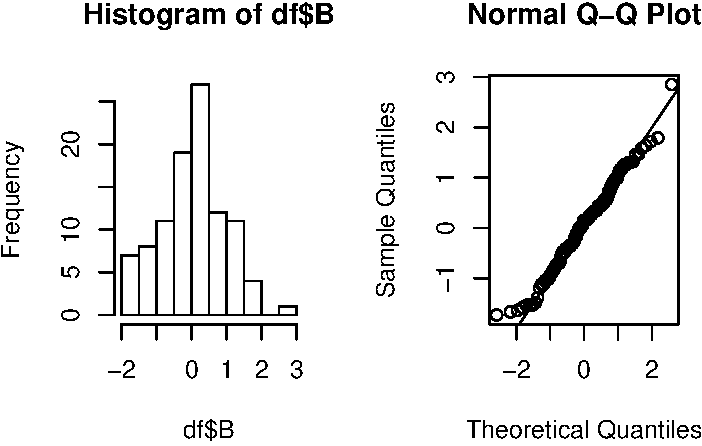
\includegraphics{04_BasicAnalyses_files/figure-beamer/unnamed-chunk-5-1.pdf}

\begin{Shaded}
\begin{Highlighting}[]
\NormalTok{## Variance}
\KeywordTok{var}\NormalTok{(df}\OperatorTok{$}\NormalTok{B)}
\end{Highlighting}
\end{Shaded}

\begin{verbatim}
[1] 1.055081
\end{verbatim}

\begin{Shaded}
\begin{Highlighting}[]
\KeywordTok{var}\NormalTok{(df}\OperatorTok{$}\NormalTok{C)}
\end{Highlighting}
\end{Shaded}

\begin{verbatim}
[1] 0.9021801
\end{verbatim}

\end{frame}

\section{ANOVA}\label{anova}

\begin{frame}[fragile]{Analysis of Variance}

The Analysis of Variance (ANOVA) is highly related to t-tests but can
handle 2+ groups.

\begin{enumerate}
\def\labelenumi{\arabic{enumi}.}
\tightlist
\item
  Provides the same p-value as t-tests
\item
  \(t^2\) = \(F\)
\end{enumerate}

For example:

\begin{Shaded}
\begin{Highlighting}[]
\NormalTok{fit_ano =}\StringTok{ }\KeywordTok{aov}\NormalTok{(df}\OperatorTok{$}\NormalTok{B }\OperatorTok{~}\StringTok{ }\NormalTok{df}\OperatorTok{$}\NormalTok{A)}
\KeywordTok{summary}\NormalTok{(fit_ano)}
\end{Highlighting}
\end{Shaded}

\begin{verbatim}
            Df Sum Sq Mean Sq F value Pr(>F)
df$A         1   0.17  0.1708   0.161   0.69
Residuals   98 104.28  1.0641               
\end{verbatim}

\begin{Shaded}
\begin{Highlighting}[]
\KeywordTok{t.test}\NormalTok{(df}\OperatorTok{$}\NormalTok{B }\OperatorTok{~}\StringTok{ }\NormalTok{df}\OperatorTok{$}\NormalTok{A)}\OperatorTok{$}\NormalTok{p.value}
\end{Highlighting}
\end{Shaded}

\begin{verbatim}
[1] 0.6890044
\end{verbatim}

\end{frame}

\begin{frame}[fragile]{Analysis of Variance}

\begin{Shaded}
\begin{Highlighting}[]
\NormalTok{fit_ano =}\StringTok{ }\KeywordTok{aov}\NormalTok{(df}\OperatorTok{$}\NormalTok{B }\OperatorTok{~}\StringTok{ }\NormalTok{df}\OperatorTok{$}\NormalTok{A)}
\KeywordTok{summary}\NormalTok{(fit_ano)}
\KeywordTok{t.test}\NormalTok{(df}\OperatorTok{$}\NormalTok{B }\OperatorTok{~}\StringTok{ }\NormalTok{df}\OperatorTok{$}\NormalTok{A)}\OperatorTok{$}\NormalTok{p.value}
\end{Highlighting}
\end{Shaded}

Notice in the code:

\begin{itemize}
\tightlist
\item
  We assigned the \texttt{aov()} the name \texttt{fit\_ano} (which we
  could have called anything)
\item
  We used the \texttt{summary()} function to see the F and p values.
\item
  We pulled the p-value right out of the \texttt{t.test()} function.
\end{itemize}

\end{frame}

\begin{frame}{Types}

\huge

\begin{enumerate}
\item One-Way
\item Two-Way (Factorial)
\item Repeated Measures
\item A combination of Factorial and Repeated Measures
\end{enumerate}

\end{frame}

\begin{frame}[fragile]{Types}

We will use the following data set for the examples:

\begin{Shaded}
\begin{Highlighting}[]
\NormalTok{df <-}\StringTok{ }\KeywordTok{data.frame}\NormalTok{(}\StringTok{"A"}\NormalTok{=}\KeywordTok{sample}\NormalTok{(}\KeywordTok{c}\NormalTok{(}\DecValTok{0}\NormalTok{,}\DecValTok{1}\NormalTok{), }\DecValTok{100}\NormalTok{, }\DataTypeTok{replace =} \OtherTok{TRUE}\NormalTok{),}
                 \StringTok{"B"}\NormalTok{=}\KeywordTok{rnorm}\NormalTok{(}\DecValTok{100}\NormalTok{),}
                 \StringTok{"C"}\NormalTok{=}\KeywordTok{rnorm}\NormalTok{(}\DecValTok{100}\NormalTok{),}
                 \StringTok{"D"}\NormalTok{=}\KeywordTok{sample}\NormalTok{(}\KeywordTok{c}\NormalTok{(}\DecValTok{1}\OperatorTok{:}\DecValTok{4}\NormalTok{), }\DecValTok{100}\NormalTok{, }\DataTypeTok{replace =} \OtherTok{TRUE}\NormalTok{))}
\NormalTok{df}
\end{Highlighting}
\end{Shaded}

\begin{verbatim}
    A            B            C D
1   0  1.815164862 -0.745933298 3
2   1  0.319942259 -0.761285771 4
3   0 -0.607921175 -0.141720206 4
4   0 -0.784290115 -0.205211852 4
5   0 -1.651797059  1.461840525 2
6   0  0.711887211 -0.003306458 1
7   0 -0.108334007  0.340000502 3
8   0  0.502882891  0.622497804 1
9   1 -1.732095717  0.122020327 1
10  1  0.640113292  0.701970372 4
11  0 -2.152221771  1.565455715 2
12  0  0.110915289 -0.358631327 1
13  1 -0.071236303 -0.427373769 3
14  0  1.227222187  0.570616653 1
15  0  1.167808604 -1.215520374 1
16  0  0.522635289 -1.557796347 2
17  0 -0.699028615 -0.132777569 1
18  0  0.940722439 -0.370254489 1
19  1  1.195203229  1.116510275 4
20  1  0.430834556  0.356613775 4
21  1 -0.042028467 -0.084611370 1
22  1 -0.728303670 -0.256821517 4
23  0  0.138753657  1.730243646 2
24  0  0.368044236 -0.144440193 2
25  1  1.059961285 -1.377942089 4
26  0  1.073189182 -0.557320326 3
27  0  0.080649512  0.328287686 2
28  1  1.480581637  1.905886074 1
29  1 -0.143013010  2.011792763 3
30  0 -1.278278559 -0.549803288 2
31  1 -0.454306566 -1.250557062 4
32  1  0.133500626 -0.213237237 3
33  0  1.215599776 -0.422934401 3
34  0  0.211433189 -0.549883329 2
35  1 -0.369465132 -0.296761894 3
36  0 -1.196516495  0.995219197 3
37  1  0.153654373  0.366781982 4
38  0  0.284317943 -1.724789759 1
39  0 -0.502050993 -0.194089851 4
40  1 -1.787376064 -0.230366098 4
41  1  0.542340047  1.861171264 1
42  1  0.022335018  0.666309028 1
43  0 -0.937623735  0.170078641 2
44  0  0.039676646 -0.315667988 2
45  0  0.439689313  0.152897968 4
46  0  1.772067616 -0.894763994 1
47  1  1.110592263 -2.037213626 4
48  0  2.473042188  0.092411813 4
49  0 -1.021211187 -1.344727047 4
50  1 -0.333723434  1.026923868 2
51  1 -0.479140290 -0.190253390 2
52  0 -0.921301456  0.631736575 2
53  0 -0.554177137  0.215630492 2
54  1 -0.534034069  0.898659600 4
55  0  0.816136291 -0.218179232 1
56  0  1.025298331  0.406088140 3
57  1  1.241516767  1.845748769 2
58  1 -0.791023287 -0.818915665 1
59  0  2.043155968  0.659283584 3
60  1 -0.755922571 -0.937895483 2
61  0  0.320656293 -0.047642195 4
62  0 -0.308383080  0.237803682 3
63  0 -0.188908362  0.354748345 2
64  1  0.663520989  1.666665869 1
65  0 -1.064291185 -1.921080433 4
66  1 -0.752429001  0.015945337 2
67  1  1.048957831  1.578515542 3
68  0  1.835893168 -0.478113588 4
69  0  0.560035479  0.698916962 2
70  1  0.764129490  0.322550667 1
71  1 -2.186750219  1.109031047 1
72  1 -0.868037913  0.570427351 4
73  1  0.305743551  0.443059977 3
74  1 -1.037171704  1.433072314 4
75  1 -1.038663796 -0.951330333 3
76  1 -1.200222400 -0.214222336 4
77  1 -1.020180932  0.068325915 2
78  1  0.086137386 -0.680132504 3
79  1  0.932248454  0.871543825 4
80  1  1.054567421 -0.620047238 3
81  1  0.281002132 -0.083097568 4
82  1  1.853731706  1.266729117 4
83  0  0.063102972  2.262451643 3
84  0 -0.837135128 -0.484147619 2
85  0  0.450716907 -1.863395539 1
86  0  1.116058831  0.372450552 3
87  1  1.157106004 -0.855179186 2
88  0  0.471329913 -1.411930152 1
89  0  0.179240750 -0.570905274 4
90  1  1.042067112 -2.022280017 2
91  1  0.878128246 -1.049342227 4
92  0  0.113085120  0.316384920 3
93  1  0.333464335  0.716905646 4
94  0 -0.327272005 -0.498340349 4
95  0  0.578433202  0.380410016 3
96  0 -0.292868130  1.356330630 4
97  1  2.885170702  0.667464323 1
98  0 -1.013578085 -1.374544766 1
99  0  1.209232260 -0.831445001 1
100 1  0.008256084 -0.268560995 1
\end{verbatim}

\end{frame}

\begin{frame}[fragile]{One-Way}

A One-Way ANOVA can be run using \texttt{aov()}.

\begin{Shaded}
\begin{Highlighting}[]
\NormalTok{fit1 =}\StringTok{ }\KeywordTok{aov}\NormalTok{(B }\OperatorTok{~}\StringTok{ }\NormalTok{D, }\DataTypeTok{data =}\NormalTok{ df)}
\KeywordTok{summary}\NormalTok{(fit1)}
\end{Highlighting}
\end{Shaded}

\begin{verbatim}
            Df Sum Sq Mean Sq F value Pr(>F)
D            1   0.08  0.0760   0.076  0.783
Residuals   98  97.40  0.9939               
\end{verbatim}

\end{frame}

\begin{frame}[fragile]{Two-Way}

A Two-Way ANOVA uses essentially the exact same code with a minor
change---including the other variable in an interaction.

\begin{Shaded}
\begin{Highlighting}[]
\NormalTok{fit2 =}\StringTok{ }\KeywordTok{aov}\NormalTok{(B }\OperatorTok{~}\StringTok{ }\NormalTok{D }\OperatorTok{*}\StringTok{ }\NormalTok{A, }\DataTypeTok{data =}\NormalTok{ df)}
\KeywordTok{summary}\NormalTok{(fit2)}
\end{Highlighting}
\end{Shaded}

\begin{verbatim}
            Df Sum Sq Mean Sq F value Pr(>F)
D            1   0.08  0.0760   0.075  0.785
A            1   0.08  0.0825   0.081  0.776
D:A          1   0.10  0.1029   0.102  0.751
Residuals   96  97.21  1.0126               
\end{verbatim}

The \texttt{D:A} line highlights the interaction term whereas the others
show the main effects.

\end{frame}

\begin{frame}{Repeated Measures}

\end{frame}

\begin{frame}{Combination}

\end{frame}

\begin{frame}{Checking Assumptions}

\end{frame}

\section{Linear Regression}\label{linear-regression}

\begin{frame}

\centerline{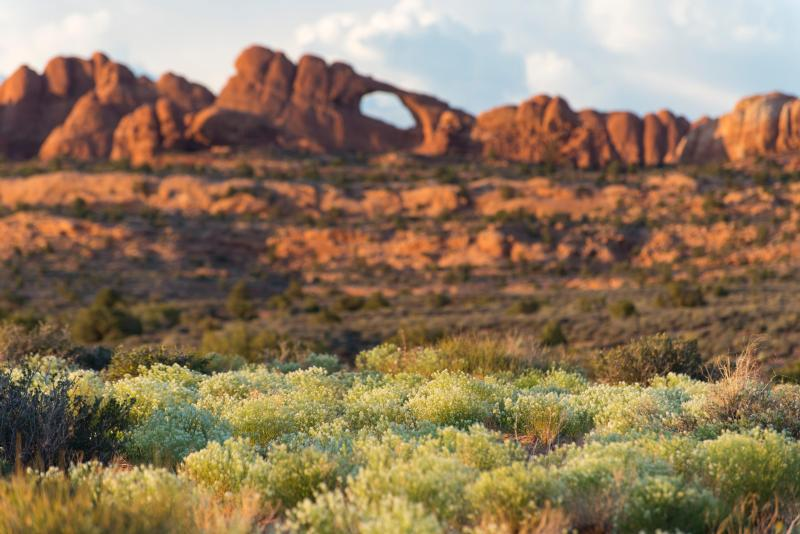
\includegraphics[height=7in]{Figures/grass_landscape_arch.jpg}}

\end{frame}
